\documentclass{VUMIFPSbakalaurinis}
\usepackage{algorithmicx}
\usepackage{algorithm}
\usepackage{algpseudocode}
\usepackage{amsfonts}
\usepackage{amsmath}
\usepackage{bm}
\usepackage{caption}
\usepackage{color}
\usepackage{float}
\usepackage{graphicx}
\usepackage{listings}
\usepackage{subfig}
\usepackage{url}
\usepackage{wrapfig}
\usepackage[table,xcdraw]{xcolor}
\usepackage[backend=biber]{biblatex}
\usepackage{enumitem}\setlist{nosep}

% Titulinio aprašas
\university{Vilniaus universitetas}
\faculty{Informatikos institutas}
\department{Programų sistemos}
%\papertype{Bakalauro darbas}
\papertype{Bakalauro baigiamojo darbo planas}
\title{Sustiprinto mokymosi taikymas žaidimo agento valdymo programos kūrimui}
\titleineng{Application of reinforcement learning to the software development for game agent management}
\author{Jokūbas Rusakevičius}
\supervisor{<reikia parašyti pareigas> Virginijus Marcinkevičius}
\reviewer{}
\date{Vilnius – \the\year}

% Nustatymai
\setmainfont[ItalicFont 	= Palem3.2-it.ttf,
			BoldItalicFont	=Palem3.2-bi.ttf,
			BoldFont		=Palem3.2-bd.ttf]
			{Palem3.2-nm.ttf}

\begin{document}
\maketitle

\setcounter{page}{2}


\subsectionnonum{Tyrimo objektas ir aktualumas}



\subsectionnonum{Darbo Tikslas, keliami uždavyniai ir laukiami rezultatai}
Šio darbo \textbf{tikslas} - \par

Darbui iškelti \textbf{uždavyniai}:\par

\begin{enumerate}
	\item Paruošti eksperimentinę aplinką ir įrašų rinkinį eksperimentui.
	\item Aptikti ir analizuoti anomalijas įrašų rinkinyje naudojantis „MacroBase“.
	\item Palyginti aptinkamamas anomalijas, keičiant įrašų rinkinio gerinimo kriterijus.
	\item Pateikti rekomendacijas IPSS duomenų anomalijų aptikimui naudojantis „MacroBase“.
\end{enumerate}

Darbo metu laukiami \textbf{rezultatai}:

\begin{enumerate}
	\item Paruošta eksperimentinė aplinka ir paruoštas darbui tinkamas įrašų rinkinys.
	\item Aptiktos anomalijos, naudojantis „MacroBase“.
	\item Pakeisti duomenys pagal tam tikrus kriterijus ir gautos tikslesnės anomalijos.
	\item Pateiktos rekomendacijos IPSS duomenų anomaljų aptikimui naudojantis „MacroBase“.
\end{enumerate}

\subsectionnonum{Tyrimo metodas} 
Darbui atlikti bus naudojami šie tyrimo metodai:

\begin{enumerate}
	\item \textbf{Mokslinės lteratūros analizė}.
	\item \textbf{Eksperimetas}.
	\subitem \textbf{Kiekybinis metodas} - aptikti pirmines anomalijas, jų priklausomybes nuo kitų atributų. Atliekamas, su visais turimais įrašų rinkiniais, ir ieškoma didžiausio anomalijų kiekio tarp turimų rinkinių.
	\subitem \textbf{Kokybinis metodas} - su turima atrinkta (arba visa) įrašų rinkinio dalimi, atliekamos įvairios manipuliacijos ir stebimi pakitimai gaunamų anomalijų tikslume priklausomai nuo padarytų pakeitimų. 
	\item \textbf{Gautų duomenų ir rezultatų analizė}.
\end{enumerate}

\subsectionnonum{Numatomas darbo atlikimo procesas}
Kaip jau minėta anksčiau, darbo eksperimentas bus atliekamas per dvi dalis, tačiau visas darbo procesas susidės iš daugiau dalių:

\begin{enumerate}
	\item Visų pirma, eksperimentui atlikti bus paruošta eksperimentinė aplinka (tikėtina Ubuntu operacinė sistema įdiegta virtualioje mašinoje).
	\item Duomenų paruošimas bus atliekamas, atrenkant svarbius tyrimui atributus ir padarant rinkinį pasiekiamą „MacroBase“ įrankiui.
	\item Jei visas įrašų rinkinys bus per didelis analizei, bus ieškoma didžiausios anomalijų dalies bandymų keliu.
	\item Su šiuo punktu, prasidės pagrindinė eksperimento dalis. Bus ieškoma ir eksperimentuojama su metodais, kurie pagerintų anksčiau gautus rezultatus.
	\item Galutinė analizė visų atliktų tyrimų ir gautų rezultatų.
	\item Pateikiama rekomendacija, kaip pagerinti anomalijų aptikimą IPSS įrašų rinkiniui naudojantis „MacroBase“ analitinį įrankį.
\end{enumerate}


\subsectionnonum{Darbui aktualūs literatūros šaltiniai}

\begin{enumerate}
	\item \textbf{\cite{macrobase_overview}} - Standfordo Universiteto išleistas straipsnis apie jų vystomą „MacroBase“ analitinį įrankį bei jo apžvalga. Šiame leidinyje yra pristatomas pats įrankis, paaiškinamas kiekvienas iš jo naudojamų darbo proceso aspektų bei principų. Tai svarbus šalitinis naudojantis „MacroBase“.
	\item \textbf{\cite{prioritizing_attention}} - Standfordo Universiteto išleistas straipsnis. Šiame leidinyje yra rašoma daugiau apie pačius principus ir teoriją, o ne apie  „MacroBase“ analitinį įrankį.
	\item \textbf{\cite{asap}} - Standfordo Universiteto straipsnis apie laiko intervalu fiksuojamus duomenis bei jų išlyginimą, padaryma lengviau skaitomais. Straipsnyje tai vadinama ASAP, analitiniu operatoriumi, kuris automatiškai išlygina įrašų rinkinį, taip padidinant analizuojamų duomenų gautų rezultatų tikslumą, bei sumažinant skaičiavimams reikalingą greitį.
\end{enumerate}




%\section{Medžiagos darbo tema dėstymo skyriai}
%Medžiagos darbo tema dėstymo skyriuose išsamiai pateikiamos nagrinėjamos temos detalės: pradiniai duomenys, jų analizės ir apdorojimo metodai, sprendimų įgyvendinimas, gautų rezultatų apibendrinimas.

%Medžiaga turi būti dėstoma aiškiai, pateikiant argumentus. Tekste dėstomas trečiuoju asmeniu, t.y. rašoma ne „aš manau“, bet „autorius mano“, „autoriaus nuomone“. Reikėtų vengti informacijos nesuteikiančių frazių, pvz., „...kaip jau buvo minėta...“, „...kaip visiems žinoma...“ ir pan., vengti grožinės literatūros ar publicistinio stiliaus, gausių metaforų ar panašių meninės išraiškos priemonių. Skyriai gali turėti poskyrius ir smulkesnes sudėtines dalis, kaip punktus ir papunkčius.

%\subsection{Poskyris}
%Citavimo pavyzdžiai: cituojamas vienas šaltinis \cite{PvzStraipsnLt}; cituojami keli šaltiniai \cite{PvzStraipsnEn, PvzKonfLt, PvzKonfEn, PvzKnygLt, PvzKnygEn, PvzElPubLt, PvzElPubEn, PvzMagistrLt, PvzPhdEn}.

%\subsubsection{Skirsnis}
%\subsubsubsection{Straipsnis}
%\subsubsection{Skirsnis}
%\section{Skyrius}
%\subsection{Poskyris}
%\subsection{Poskyris}

%\sectionnonum{Rezultatai ir išvados}
%Rezultatų ir išvadų dalyje išdėstomi pagrindiniai darbo rezultatai (kažkas išanalizuota, kažkas sukurta, kažkas įdiegta), toliau pateikiamos išvados (daromi nagrinėtų problemų sprendimo metodų palyginimai, siūlomos rekomendacijos, akcentuojamos naujovės). Rezultatai ir išvados pateikiami sunumeruotų (gali būti hierarchiniai) sąrašų pavidalu. Darbo rezultatai turi atitikti darbo tikslą.

\printbibliography[heading=bibintoc]  % Šaltinių sąraše nurodoma panaudota
% literatūra, kitokie šaltiniai. Abėcėlės tvarka išdėstomi darbe panaudotų
% (cituotų, perfrazuotų ar bent paminėtų) mokslo leidinių, kitokių publikacijų
% bibliografiniai aprašai. Šaltinių sąrašas spausdinamas iš naujo puslapio.
% Aprašai pateikiami netransliteruoti. Šaltinių sąraše negali būti tokių
% šaltinių, kurie nebuvo paminėti tekste. Šaltinių sąraše rekomenduojame
% necituoti savo kursinio darbo, nes tai nėra oficialus literatūros šaltinis.
% Jei tokių nuorodų reikia, pateikti jas tekste.

% \sectionnonum{Sąvokų apibrėžimai}
%\sectionnonum{Santrumpos}
%Sąvokų apibrėžimai ir santrumpų sąrašas sudaromas tada, kai darbo tekste vartojami specialūs paaiškinimo reikalaujantys terminai ir rečiau sutinkamos santrumpos.

%\appendix  % Priedai
% Prieduose gali būti pateikiama pagalbinė, ypač darbo autoriaus savarankiškai
% parengta, medžiaga. Savarankiški priedai gali būti pateikiami ir
% kompaktiniame diske. Priedai taip pat numeruojami ir vadinami. Darbo tekstas
% su priedais susiejamas nuorodomis.

%\section{Niauroninio tinklo struktūra}
%\begin{figure}[H]
%    \centering
%    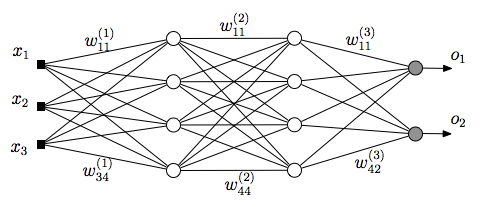
\includegraphics[scale=0.5]{img/MLP}
%    \caption{Paveikslėlio pavyzdys}
%    \label{img:mlp}
%\end{figure}


%\section{Eksperimentinio palyginimo rezultatai}
% tablesgenerator.com - converts calculators (e.g. excel) tables to LaTeX
%\begin{table}[H]\footnotesize
%  \centering
%  \caption{Lentelės pavyzdys}
%  {\begin{tabular}{|l|c|c|} \hline
%    Algoritmas & $\bar{x}$ & $\sigma^{2}$ \\
%    \hline
%    Algoritmas A  & 1.6335    & 0.5584       \\
%    Algoritmas B  & 1.7395    & 0.5647       \\
%    \hline
%  \end{tabular}}
%  \label{tab:table example}
%\end{table}

\end{document}
